 \documentclass[12pt]{article} % bigger font

% Essential packages
\usepackage[T1]{fontenc}
\usepackage[utf8]{inputenc}
\usepackage{lmodern}

\usepackage{amsmath,amssymb,amsfonts}
\usepackage{graphicx}

% Keep default margins → no geometry package

% Line spacing
\usepackage{setspace}
\setstretch{1.3} % slightly airy but not too loose

% Paragraph style
\setlength{\parindent}{0pt}
\setlength{\parskip}{0.6em}

% Slightly increase line height globally
\linespread{1.05}

% Math commands
\newcommand{\field}[1]{\mathbb{#1}}
\newcommand{\R}{\mathbb{R}}
\newcommand{\C}{\mathbb{C}}
\newcommand{\Z}{\mathbb{Z}}

\newcommand{\de}{\mathrm{d}}
\newcommand{\dt}{\mathrm{d}\theta}

% Section formatting with better spacing
\usepackage{titlesec}

\titleformat{\section}
  {\centering\large\bfseries}
  {\thesection}{1em}{}

\titlespacing{\section}
  {0pt}{2em}{0.8em}

\titleformat{\subsection}
  {\normalsize\bfseries}
  {\thesubsection}{1em}{}

\titlespacing{\subsection}
  {0pt}{1.5em}{0.5em}

% Page numbering
\pagestyle{plain}

% Abstract formatting (less cramped)
\renewenvironment{abstract}
 {\small
  \begin{center}
  \bfseries \abstractname\vspace{0.3em}
  \end{center}
  \list{}{%
    \setlength{\leftmargin}{3mm}
    \setlength{\rightmargin}{3mm}
  }%
  \item\relax}
 {\endlist}

\begin{document}

\title{\Large\textbf{Representation in $\mathbb{R}^{\,3}$ of a not yet metric\,-\,possessing Trace by an Ensemble: Curve\,-\,Evolute.}}          
\author{Giuseppe G. Lamberti\\
\small LMBGPP34L27D742Z\\
\small email: giuse.lamberti@gmail.com}
\date{2026}

\maketitle

\begin{abstract}
\begin{small}
\noindent An enlarged concept of Curve is introduced. Not only expressed by Curvature and Torsion, but by Rotations: around the Curvature Centers, and around T, N, B of the Frenet-Serret frame.

\noindent Stationary in $\mathbb{R}^{3}$, not yet expressed by the Euclidean metric hence called bare, a Trace is analyzed by an ordered set of Triangles, corresponding to a set of Planes, obtaining an Ensemble: Curve\,+\,Evolute. The Triangles are exactly bounded by the Curve's and Evolute's components; a Triangulation Nest in $\mathbb{R}^{\,3}$ becomes the final Reference Space for the Ensemble. The result is an Intrinsic Description of the Ensemble.

\noindent Program CPlanes.py is enclosed. Its Layer 1 assists the Trace's intrinsic parametrization; its Layer 2 analyzes the Trace's properties.      
\end{small}
\end{abstract}

\begin{center}
\bfseries{Notation}
\end{center}

\noindent \textsl{The following Notation is for the Text.\\ The Program has, and explains, its own Notation.} 

\noindent \{Curve's Parameter\} = \{\,t\,\}\,.

\noindent Index = \{\,i\,\}\,, (a low index).

\noindent \{Curve's Parameter\} , \{Marks' Index\} have same Direction and Orientation. 

\noindent Odd index\; for any \{\,Curve Triangle\,\}\,=\,$\Gamma$\,.

\noindent Even index\; for any \{\,Evolute Triangle\,\}\,=\,$\Lambda$\,.

\noindent Same odd index for \{Curve Plane\}, \{Curve Triangle\}, Arc,  Arc's Curvature Center, Arc's scalar Radius, Arc's Intermediate MarK.

\noindent Same even index for \{Evolute Plane\}, \{Evolute Triangle\}
and its unique Mark.
 
\noindent In a Triad a Vector Radius is expressed by two low indices: the 1st indicates the tip Mark = $p_{\,i}$\;,\;the 2nd indicates the root \{Curvature Center\} = $C_{\,j}$. \\Vector Radius \;$R_{\,i\;j} = [\,p_{\,i} - C_{\,j}\,]$\,.

\noindent Unit Vectors\, \textsl{at an Even Mark} = $p_{\;j}$ \,are  expressed:

 incoming $T_{\,p_{\;j}}$ = $T_{\,\to\,p_{\;j}}$\quad , \quad outgoing $T_{\,p_{\;j}}$ = $T_{\,p_{\;j}\,\to}$
 
 incoming $N_{\,p_{\;j}}$\quad        , \quad outgoing $N_{\,p_{\;j}}$
 
 incoming $B_{\,p_{\;j}}$\quad, \quad outgoing $B_{\,p_{\;j}}$ = $B_{\,p_{\;j}\,\to}$
  
Where: incoming from the\; \textsl{previous} \{Curve Arc\},\\ outgoing to the\; \textsl{next} \{Curve Arc\}.

\noindent Mark = evidenced Point, common to Trace and Curve.\\ Any Curve's Mark is parametrized and indexed.

\noindent The set \{\,Marks\,\} is linearly ordered by the Index:  

\noindent Indexed Set \{\,Marks\,\} = $\{\,p_{\,i}\,\}$\,;\quad $p_{\,0} \leq p_{\,i} \leq p_{\,n}$

\noindent Even Mark = EM, with an even index ; Odd Mark = OM, with an odd index.

\noindent Boundary Marks (\,two\,) of an Arc. with even indexes.

\noindent Intermediate Mark (\,one\,) of an Arc. With odd index.

\noindent Oriented Mark =  $p_{\;j}\;=\;\to\,p_{\;j} +\, p_{\;j}\,\to$

\noindent Common Mark, for a sequence of Triangles; with even index:\\ \big\{\;\{Curve Triangle\}, \{Evolute Triangle\}, \{Curve Triangle\}\;\big\} = \{\,Tern\,\}.\\The Common Mark is a Point of each Triangle. 

\noindent Triad's Curvature Center = Arc's Curvature Center
 = Evolute's Point = $C_{\,i}$\,,\\ where i = Triad's and Arc's odd index.

\noindent ||\;Distance between the generic Points q, p\;|| = $d_{\;q\,p} \vee ||\,d\;q\,p\,|| = ||\,p\,-\,q\,||$\,.

\noindent Root = p\,, Tip = q . Vector = $[\;p -q\;]$\,.

\noindent $ \{Reference\;Marks\} = qs = \{\,q0, q1, q2, q3\,\}$.

\noindent Associated to the chosen, unique subset \{\,Reference Marks\,\} = qs\,,\\ the set \{\,Reference Distances\,\}: 

\noindent d00 = ||\,q0 - q0\,||\,, d01 = ||\,q1 - q0\,||\,, d02 = ||\,q2 - q0\,||\,, d03 = ||\,q3 - q0\,||\,.

\noindent d12 = ||\,q2\,-\,q1\,||\,, d13 = ||\, q3\,-\,q1\,||\,, d23 = ||\,q3\,-\,q2\,||\,; 

\noindent For the \{\,Reference Marks\,\}:

\noindent \{\,Triples\,\} = \big\{\,\{q0, q1, q2\}, \{q1, q0, q3\}, \{q0, q2, q3\}, \{q2, q1, q3\}\,\big\}. 

\noindent Each Triple of Reference Marks defines one \{Base Plane\}.

\noindent Each Oriented Triple defines an \{Oriented Base Plane\}.

\noindent \textbf{Function} $f(\,t\,)$\,.\quad We distinguish, for a function f\,(t), the cases:
  
\noindent a) The abrupt, \textsl{local} at $(\,i\,)$ change:\; $f\,(\,t_{\;\to\,p_{\;i}}\,)$\;\;-->\;\;$f\,(\,t_{\;p_{\;i}\;\to}\,)$\,.

\noindent b) The differential from $f(\,t\,)$ \,to \,$f(\,t + d\,t\,)$\,. 

\noindent Triangles.\, \{\,Curve Triangle\,\} = $\Gamma$\;.\;\{\,Evolute Triangle\,\} = $\Lambda$\,.
 
\noindent Different symbols for them, but an uninterrupted Ordered Set of values of the index.

\noindent \{\,D C M\,\} = \{\,Direction Cosine Matrix\,\}.

\noindent \{\,T, N, B\,\} = Frenet - Serret frame of Unit Vectors.

\noindent \{\,Tern\,\}$_{\;i-1}$ = Ensemble's sequence:\\ \big\{\;\{Curve Triangle\}$_{\,i-2}$, \{Evolute Triangle\}$_{\,i-1}$, \{Curve Triangle\}$_{\,i}$\;\big\}.

\noindent With even index (\,i-1\,).
 
\noindent \{\,Triad\,\} = a sequence of 3 Marks.

\section{Trace}

\noindent Previously the Human ascertained the Euclidean Geometry of the part of space in which the Trace lies. 

\noindent Stationary being independent of $\mathbb{R}^{\,0}$ in $\mathbb{R}^{\,3+1}$, and not yet expressed by the Euclidean metric, a Trace, a.k.a. Shape, is given and perceived by an operating in $\mathbb{R}^{\,3+1}$ Human Observer. That is, a deformable Trace in $\mathbb{R}^{\,3+1}$ is not considered here.
The considered Trace is not a Set of disjoint Points; its Points are sensibly connected into the Trace itself. Hence the Trace has \textsl{Positional Continuity}. Generally it can have other types of geometric Continuity\,/\,Discontinuity. It is not, but it shall be transformed into an \{\,Ensemble: Curve + Evolute\,\}. It can be either regular or not regular, open or closed, with coexisting left-handed and right-handed pieces.  It is the \textsl{Datum} of the Human's analysis. In this analysis, it is not stretched, not smoothed by the Human. In the Representation by said Ensemble it is associated to Measures, Marks, an Index, a Parameter, a Reference Space.

\noindent There is a set of possible Definitions of a Trace.
A preliminary extrinsic definition in $\mathbb{R}^{\,3}$ is not introduced here.

\noindent An Intrinsic Definition of the ensuing Ensemble is given by a Reference Space, that, completed at the analysis' end, is a \{\,Triangulation Nest\,\} in $\mathbb{R}^{\,3}$, each Triangle being stationary and stationarily connected to the other Triangles.  

\noindent \textbf{Trace's Resolution of its geometric features.} It depends on how finely the Human samples the Trace. It is a Human's choice with phisical limitations, like the Human's size in relation to the Trace, her available sensors, the smallest features of interest, the required level of detail. In general it varies from place to place in the Trace.

\noindent \textbf{Precision of the Representation:} it is proportional to the assumed density of Marks.  

\section{Marked Trace}

\noindent The Human performs preliminary operations on the Trace:

\noindent She perceives on the Trace a set \{\,not yet parametrized Points\,\}. (2.1)

\noindent She conceives a \textbf{\textsl{Direction}} along the Trace: the Linear Direction. (2.2)
 
\noindent She chooses a specified \textsl{\textsl{Orientation}} for this Direction; one within two. (2.3)

\noindent To the Trace, she affixes, after pondered thoughts, an Ordered Set \; \textsl{\{\,Marks\,\}\,=\\ \{\,Marked Trace's noticeable Points, suitably chosen for its Representation\,\} $\subset$ \{\,Trace's Points\,\}.} \qquad (2.4)  

\noindent Hence the ensuing \{\,Marked Trace\,\} has a specified, indexed but not parametrized set (\,the Curve shall be parametrized\,)\\ 
\textsl{Directed \& oriented \{\,Marked Trace's Evidenced Points\,\} = \{\,Marks\,\}.}

\noindent \textbf{Sequences on a Marked Trace.} An \textsl{appropriate, Sequence} of indexed Marks must be assumed, and kept carefully, since the two subsets of \{\,Marks\,\}: \{\,Even Marks\,\} = \{EMs\}, \{\,Odd Marks\,\} = \{OMs\}, have different functions. \quad  (2.6)

\noindent a\,) Sequence of Marked Trace's Marks:\\\big\{\;\{EM\} ,\,....\,,\{EM\} , \{OM\} , \{EM\} ,\,....\,,\{EM\}\;\big\};

\noindent here it is written: \quad \{\,Marks\,\} = $\{\,p_{\,0}\,,\,....\,,\,p_{\,i-1}\,,\,p_{\,i}\,,\,p_{\,i+1}\,,\,....\,,\,p_{\,n}\,\}$\,.\\ Where: \, $p_{\,0}\,,\,...\,,\,p_{\,i-1}\,,\,p_{\,i+1}\,,\,...\,,p_{\,n}$ \; are Even Marks.\qquad (2.7)

\noindent b\,) Sequence of Marked Trace's Intervals:\\ $\big\{\;....\,,\,\{\,p_{\,(i-1)\,\to}\,\,,\,...\,,\,p_{\,(\,i)}\,,\,...\,,\,p_{\,\to\,(i+1)}\,\}\,,\,...\;\big\}$. \qquad (2.18)

\noindent \textbf{Marked Trace's Intervals.} If not with an angle near $\pi$, any Marked Trace's Interval with constant or nearly constant Curvature, and negligible other Rotations, must be conveniently fitted by two boundary \{EMs\} and one intermediate OM. \qquad (2.19) 

\noindent The above expedient of assuming three Marks and defining them the only \{\,Marks\,\} in a marked Trace's Interval with constant Curvature, is for the entire Marked Trace.\\ By this expedient the necessary No. of Marks for the Trace's Representation called Curve is reduced to a minimum. \qquad (2.20)

\noindent \textbf{\{\,Even Marks\,\}.} The Human must define the elements of the subset \{\,Even Marks\,\} = \{EMs\} of the Marked Trace. a) In a Mark, some geometric properties change abruptly. So that to define it a distinguishing EM is mandatory. b) But not necessarily an abrupt change corresponds to an EM. In one Interval, an EM with another task: the transformation of the OM into one EM, and the creation of two new OMs. Aiming to the partition of one too long Marked Trace Interval into two shorter Intervals.\qquad (2.21)  

\noindent \textbf{\{\,Odd Mark\,\}.} In the Interior of any Marked Trace's Interval that is defined by 3 Marks only. Between the two Even Marks, one, and only one

\noindent \{Intermediate Mark\} = \{\,Odd Mark\,\} = OM.  

\noindent This OM is necessary in the ensuing Curve, for the definition of: the local circular \{\,Arc\,\} and its Curvature. Not necessarily it is the \{Arc's Medium Point\}, but the precision of the analysis is enhanced if said OM is near the \{Arc's Medium Point\}. \qquad (2.22) 

\noindent In the same Marked Trace's Interval:

\noindent \textsl{\{\,Marked Trace's non-evidenced Points\,\} $\neq$ \{\,Marks\,\}.} \qquad \qquad \qquad \quad (2.23)

\noindent \textbf{Index.} The set \{\,Marks\,\} has an ordering \{\,Mark Index\,\} = \{\,i\,\},

\noindent hence the \{\,Marked Trace\,\} has \{\,Mark Index\,\}. \;\qquad (2.24)

\noindent Marked Trace's \{\,Marks\,\} are indexed but not yet parametrized, by definition. \qquad (2.25)

\textbf{Accuracy.} The Representation of the \{\,Trace\,\} by an ensuing \{\,Curve\,\} is accurate if Human's attention to abrupt changes and smooth changes is applied in the transformation of the \{\,Trace\,\} into a \{\,Marked Trace\,\}. \qquad (2.26)

 \section{Curve}
 
\noindent \textbf{\{\,Curve\,\}.} A \{\,Curve\,\} is a Human\,-\,conceived Representation of a given \{\,Trace\,\}. In this study the process of Trace's Representation is:\\Trace -> Marked Trace -> Curve --> Ensemble.  
  
\noindent \textbf{\{Regular Curve\}.} Math coontains the concept of \{Regular Curve\}.
  
\noindent \textbf{\{Non-regular Curve\}.} Here, the superposed pieces of a \{Non-regular Curve\} are analyzed locally and separately. This is possible since the elements (\,Points, Arcs, Rays, Vectors, Planes, Triads, Tetrads, Terns\,) of each piece are mot only parametrized and indexed in $\mathbb{R}^{\,3}$, but also linearly and distinguishably along the Curve. So that the analysis of one piece ignores the other superposed pieces. \qquad \qquad (3.1)

\noindent \textbf{Generic Curve.} A generic Curve may have: Abrupt change Marks, finite Arcs and differential Arcs. \qquad (3.2)

\noindent\textbf{\{\,Marks\,\}.}\qquad \textsl{\{\,Marks\,\}\,=\,\{\,Indexed Points\,\} =\\ \{Marked Trace's Evidenced Points\}\,=\,\{Curve's Evidenced Points\}.}  

\noindent \{Marked Trace\} and ensuing \{Curve\} coincide obligingly only at the Marks. 

\noindent The \{\,Marked Trace's Marks\,\} are assumed as \{\,Curve's Marks\,\}. (3.3)

\noindent \textbf{\{Non-evidenced Points\}.} \{\,Marked Trace's non-evidenced Points\,\} $\neq$ \{\,Marks\,\} $\neq$ \{\,Curve's non-evidenced Points\,\}. Because:

\noindent As the name tells us: \{Marked Trace non-evidenced Points\} are Marked Trace's properties. 

\noindent The \{\,Curve's non-evidenced Points\,\} lie in circular \{\,Arcs\,\} $\subset$ Curve ; generally not strictly along the Marked Trace.

\noindent \textsl{But: each Curve's circular Arc approximates a Marked Trace's Interval.} (3.4) 

\noindent The Human strives to get their nearness in $\mathbb{R}^{\,3}$. \qquad \qquad (3.5)

\noindent \textbf{Curve's Parameter.} The Human applies the \textbf{\textsl{Parameter}} \{\,t\,\} to the Curve. Each Point (\,Mark and Non-evidenced Point\,) of the Curve gets a Parameter value. \qquad (3.6)

\noindent \{\,Curve's Points\,\} = $\{\;p_{\;t}\;\}$\,. \qquad (3.7)

\noindent \{\,Curve's indexed \& parametrized Points\,\} = \{\,Curve Marks\,\} = \{\,$p_{\;i}$\,\} \qquad (3.8)

\noindent $\{\;p_{\;t}\;\} \supset \{\,p_{\;i}\,\}$\,. \qquad (3.9)

\noindent \textbf{Density of Curve's Marks.} It is relative to the Parameter.

\noindent It was said before for the Marked Trace. Where the \{\,Marks\,\} are placed thightly, the Curve varies with a sequence of short Arcs.\qquad (3.10)  

\noindent An Open Curve has Even End Marks\; $p_{\,0}\,,\,p_{\,n}$\,.\qquad (3.11)

\noindent An Open Curve that begins with one EM and ends with one OM has an incomplete and undefined final \{\,Arc\,\}.\qquad (3.12)
 
\noindent A Closed Curve has superposed Initial and Final Even Marks\; $p_{\,0}\,,\,p_{\,n}$\,. (\,Distinct indexes\,) \qquad (3.13)

\noindent \textbf{Representation of a Trace by a Curve.}\; According to the Human:

\noindent 1] By definition: one \{Marked Trace's Mark\}, and the corresponding \{Curve's Mark\}, have the same position in an assumed $\mathbb{R}^{\,3}$. (3.14)
 
\noindent 2] A \{Marked Trace's Non-evidenced Point\} is represented by the \{Curve's Non-evidenced Point\} that is in $\mathbb{R}^{\,3}$ at the minimum distance from it. (3.15)   

\noindent 3] A smooth \{Transition\} = \{change of some value\} in the Marked Trace must correspond to a smooth \{Transition\} in the Curve. \;A non-smooth Transition at a Marked Trace's EM must correspond to a non-smooth Transition at the Curve's same indexed EM. (3.16)

\noindent \textbf{\{\,Pair of Marks in sequence\,\}.} It is a Curve's component, not of the Evolute. By \{\,t\,\}, it may define a Distance
 = $\Delta^{\,1}\,t$\,. (3.17)

\noindent \textbf{\{\,Triad\,\}.} A \{Triad\} is a Curve's component, not of the Evolute.   

\noindent It is defined by a subset of 3 Marks of the Marked Trace: one in the Triad incoming EM, one intermediate OM, one from the Triad outgoing EM, and their \{\,Interval Interior\,\}, i. e. \{\,Arc Interior\,\}. Three Indexes in the Sequence \{\,Marks\,\} correspond to them. One \{\,Triad Triangle\,\} $\subset$ \{\,Triad Plane\,\}, one \{\,Triad Arc\,\} in it. And their properties. One single \{\,Triad\,\} may define a $\Delta^{\,2}\,t$\,, Curvature, but not Torsion etc. \qquad \qquad (3.18)

\noindent In the Triad's Triangle: the Arc's Curvature, and the Arc's Curvature Center that is a Triad's property and is ascribed as an Evolute's Point. \qquad \qquad (3.19) 

\noindent The introduction of \{\,Triad\,\} is due to the Points'principle, here Marks' principle too: \textsl{Always 3 distinct, not aligned Points define a Plane and in it an Arc of Circle. If the Triad has 3 distinct, aligned Points, a straight Arc is defined, but not a Plane.} (3.20)

\noindent \textbf{\{\,Tetrad\,\}.} A \{\,Tetrad\,\} is a sequence of four Points; eventually of four Marks. One Tetrad may define a $\Delta^{\,3}\,t$ and Torsion. (\,See the subsection "Differential Vectors on the Curve"\,).  (3.22)
 
 \noindent \textbf{\{\,Triads\,\}.} The ordered set \{\,Marked Trace's Marks\,\} is associated to the ordered set \{\,Marked Trace's Triads\,\}.The ordered set \{\,Curve's Marks\,\} is associated to the ordered set \{\,Curve's Triads\,\}.\qquad \qquad (3.23)

\noindent \textbf{\{\,Arc\,\}.} The \{\,Arc\,\} of a Triad is an ordered subset of Curve's \{\,Points\,\}, comprehensive of: 3 evidenced Points ( no less, no more ) called Marks (\,one Triad\,), and other non-evidenced Points. It is a Curve's Interval with a Marks-defined, constant Curvature (\,not Torsion, etc.: 3 Marks not sufficient\,)..\qquad (3.24)

\noindent In the Arc Interior, the geometric properties change smoothly, by definition. If not so, the set \{\,Marks\,\} must be reorganized. \qquad (3.25) 

\noindent \textbf{Generic Arc\,.} \;\{\,Arc\,\}$_{\;i}$ = $A_{\;i} \supset \{\;p_{\,(i-1)\,\to}\;, ... ,\;p_{\,i}\;, ... ,\;p_{\,\to\,(i+1)}\;\}$ = $\{\;Outgoing\;from\;p_{\;i-1}\;, ... ,\;p_{\;i}\;, ... ,\;Incoming\;into\;p_{\;i+1}\;\}$\,.

\noindent \{OM\} = $p_{\;i}$\,. \{EMs\} = $\{\;p_{\,(i-1)\,\to}\;\,,\,\;p_{\,\to\,(i+1)}\;\}$\,. Odd\, i \qquad \qquad \qquad (3.26)

\noindent \textbf{Arc\,-\,length.} In general, the Curve's \{\,Arcs\,\} do not have equal lengths.\qquad (3.27)

\noindent \textbf{Arc's Frenet-Serret field.} Each Arc $A_{\,i}$ has its \{\,T, N, B\,\}$_{\,A_{\,i}}$ Frenet-Serret field, bar a straight Arc $A_{\,j}$ having its $T_{\,A_{\,j}}$ field only.  (3.28)

\noindent Incoming in $Int\;A_{\,i}$\,, hence Outgoing from $p_{\,i-1}$\,:\qquad \{\,T, N, B\,\}$_{\;p_{\;(i-1)\,\to}}$\,. 

\noindent Outgoing from $Int\;A_{\,i}$\,, hence Incoming into $p_{\,i+1}$\,:  \qquad \{\,T, N, B\,\}$_{\,p_{\,\to\,(i+1)}}$\,, 

\noindent Outgoing from $p_{\,i-1}$ that is the \{\,Initial Mark\,\} of $A_{\,i}$\,: \quad \{\,T,\,N,\,B\,\}$_{\,p_{\,(i-1)\,\to}}$\;.\\Incoming into $p_{\,i+1}$ that is the \{\,Final Mark\,\} of $A_{\,i}$\,: \quad \{\,T,\,N,\,B\,\}$_{\,p_{\,\to\,(i+1)}}$\,. \qquad (3.29)

\noindent \textbf{In $A_{\,i}$\,.} For a non-straight Arc $A_{\,i}$\,. Changing Point in the Interior of $A_{\,i}$\,, for definition of Triad:\; \{\,T\,\}, \{\,N\,\}, change smoothly; \{\,B\,\} changes its \{Point of application\} only, keeping constant Direction \& Orientation. The field \{\,B\,\}$_{\,A_{\,i}}$ is perpemdicular to $A_{\,i}$\,; all its elements $B_{\,p}$ are parallel. \qquad (3.30) 

\noindent \textbf{Straight Arc\,.} A \{Straight Arc\} is a 3 - Marks - defined straight Segment. Its Curvature Center is at $\infty$\,, not in a defined Plane.\\ Its Boundary Vector Radii are parallel, not in a defined Plane.\\ Defined \{\,T\,\}\,, undefined \{\,N\,\}\,,\,\{\,B\,\}\,. \qquad (3.31)

\noindent \textbf{Degenerate Arc \#\,1}, An \{\,Arc\,\} with one EM and one OM only, or two EMs and no OM. It is incomplete and undefined. A revision of the set \{\,Marks\,\} is necessary. \qquad \qquad (3.32)

\noindent \textbf{Degenerate Arc \#\,2.} An \{\,Arc\,\} with more than 3 Marks, in general without uniform curvature. For this reason it must be decomposed. (3.33)  

\noindent \textbf{Differential Triad.} A Differential Triad has the usual 3 Marks and a tiny Arc of 2, generally not aligned, Differential Intervals. 

\noindent And as usual, also for a Differential Triad the two Boundary \{Even Marks\} = EMs and the Intermediate \{Odd Mark\} = OM define the Triad and the Index order. \qquad (3.34)

\noindent In a Differential Triad there is the advantage of defining locally the Curve uniquely by an easy to define Curvature, not by a set of elementary Rotations. \qquad (3.35)

\noindent \textbf{Sequence of Differential Triads.} Applying a big No. of Marks in a given Marked Trace Interval, and in the corresponding Curve Interval, by a Sequence of Differential Triads, the fidelity of the local Representation is enhanced.

\noindent The complication of the Trace induces a big No. of Differential Triads in Sequence (\,obviously this is an inconvenience\,). (3.36)  

\noindent \textbf{Differential Arc.} Say\,\{Arc\}$_{\,i}$\,=\,$A_{\,i}\,\supset\,\{\,p_{\,(i-1)\,\to}\;, ... ,\;p_{\,i}\;, ...\;p_{\,\to\,(i+1)}\,\}$.\\\,Odd \,i\,, with a Pair of Differential, straight Intervals. In general, non-null Curvature, hence non-straight Arc, even if of tiny length. (3.37)

\noindent \textbf{Differential Vectors on the Curve and their Points of application.}

\noindent ( An impractical symbolism is used to enhance understanding. )
 
\noindent The sum of Vectors with the same origin is considered allowable. \qquad (3.38)

\noindent It is well known that 2 Points are necessary to get a 1st differential; 3 Points to get a 2nd differential; 4 Points to get a 3rd 
differential .... \qquad (3.39)
 
\noindent\textbf{A 3rd Differential on the Curve.} Let us suppose on the Curve 4 Points:\; $t_{\,1}\,,\,t_{\,2}\,,\,t_{\,3}\,,\,t_{\,4}$ and the Differential Vectors\; $\Delta^{1}\,t_{\,1 \to 2} = [\,t_{\,2} - t_{\,1}\,]$\, applied at $t_{\,1}$\;, $\Delta^{1}\,t_{\,2 \to 3} = [\,t_{\,3} - t_{\,2}\,]$\, applied at $t_{\,2}$\,, $\Delta^{1}\,t_{\,3 \to 4} = [\,t_{\,4} - t_{\,3}\,]$\, applied at $t_{\,3}$\,. \qquad (3.40)

\noindent They are assumed straight Differential Vectors because\\ $||\,t_{\,2} - t_{\,1}\,||\;,\;||\,t_{\,3} - t_{\,2}\,||\;,\;||\,t_{\,4} - t_{\,3}\,||$\\ are very little in comparison to the local Curvature Radius. \qquad (3.41)

\noindent Changing sign, the Point of application changes; for example:

\noindent $\Delta^{1}\,t_{\,1 \to\,2}$ is applied at $t_{\,1}$\,,

\noindent  $- \Delta^{1}\,t_{\,1 \to 2} = \Delta^{1}\,t_{\,2 \to 1}$\; is applied at $t_{\,2}$ and has the tip at $t_{\,1}$\,.

\noindent A longitudinal translation\,  $\Delta^{1}\,t_{\,1\, \to\, 2} = \Delta^{1}\,t_{\,2\, \to\, a}$\,, yields:  $\Delta^{1}\,t_{\,2\,\to\, a}$\,, that is applied at $t_{\,2}$ and has the tip at\, a\,.

\noindent At $t_{\,2}$\,:\; $\Delta^{1}\,t_{\,2\,\to\, a}$\, is vectorially added to $\Delta^{1}\,t_{\,3\,\to\,2}$\,, getting $\Delta^{2}\,t_{\,3\,\to\,a}$, applied at $t_{\,3}$\,.\; (\,$\Delta^{2}\,t_{\,3\,\to\,a}$\, has the same size and direction, opposed orientation of $\Delta^{2}\,t_{\,2\,\to\,b} = \Delta^{1}\,t_{\,2\,\to\,1} + \Delta^{1}\,t_{\,2\,\to\,3}$\,, that is applied at $t_{\,2}$\,). \quad (3.42)

\noindent By the parallelogram construction of two Vectors, both with origin at $t_{\,3}$\,, we get:\; $\Delta^{\,2}\,t_{\,3\, \to\, c} = \Delta^{\,1}\,t_{\,3\, \to\, 2}\, + \,\Delta^{\,1}\,t_{\,3\, \to \,4}$\; that we say applied at\, $t_{\,3}$\,, not to\, $t_{\,2}$\,. \qquad (3.43)

\noindent $\Delta^{3}\,t_{\,3\,\to\,d} = \Delta^{2}\,t_{\,3\,\to\,a} + \Delta^{2}\,t_{\,3\,\to\,c}$\,, that we say applied at\, $t_{\,3}$\,, where there is the vectorial sum. \qquad (3.44)

\noindent \textbf{Derivatives.} By the above we get the Derivatives:\\$\Delta^{1}\,t\,/\,\Delta\,t\quad;\quad\Delta^{2}\,t\,/\,2\,\Delta\,t^{\,2}\quad;\quad\Delta^{3}\,t\,/\,6\,\Delta\,t^{\,3}$\,. \qquad (3.45)

\noindent \textbf{\{Curve Plane\}.} To each \{\,Triad\,\} and its corresponding \{\,Arc\,\}, necessarily a Plane in $\mathbb{R}^{\,3}$ corresponds. Since it contains elements of the Curve, it is named \{Curve Plane\}. \qquad \qquad (3.46)

\noindent \{Curve Plane\}$_{\;i}$ $\supset$ \{Curve Triangle\}$_{\,i}$ = $\Gamma_{\,i}$\,. \qquad  Odd i\,.\qquad \qquad (3.47)

\noindent \textbf{\{Curve Triangle\}.} say $\Gamma_{\,i}$. $\Gamma_{\,i}$ contains: the Triad, the Arc = $A_{\,i}$ with all its \{\,Points\,\} and within them its \{Triad's Marks\} = $\{\,p_{\,(i-1)\,\to}\,,\,p_{\,i}\,,\,p_{\,\to\,(i+1)}\,\}$\,, the local \{Curve Center\}$_{\,i}$ = \{Arc's Curvature Center\}$_{\,i}$ = \{Evolute Point\}$_{\,i}$ = $C_{\,i}$ that is associated to the Rotation (\,see a following subsection\,)\, $\theta\;B_{\,C_{\,i}}$\,, (\,around $B_{\,C_{\,i}}$\,, not around $B_{\,p_{\,i}}$\,) the \{Scalar Radius\} = $r_{\,i}$, common to all Points of $A_{\,i}$, the Vector Radii, one for each Point of $A_{\,i}$\,, within them the \{Initial Vector Radius\} = $R_{\,(i-1)\,(i)} = \big[\; p_{\;i-1} -\, C_{\,i}\;\big]$  and the \{Final Vector Radius\} = $R_{\,(i+1)\,(i)} = \big[\;p_{\;i+1} -\, C_{\,i}\;\big]$\,. (3.48)

\noindent \textbf{\{Curve Triangle\}'s relevants Points}:\\ one OM, two EMs, one \{Curvature Center\}. (3.49) 

\noindent \textbf{Curve's \{Initial Curve Triangle\}.} The Open $\vee$ Closed Curve's \{Initial Curve Triangle\} be $\Gamma_{\,1}$\,; OM = $p_{\,1}$\,, \{EMs\} = $\{\,p_{\,0\,\to}\;,\;p_{\,\to\,2}\,\}$\,, \{Initial Triad\,\}$_{\,1}$ = $\{\;p_{\,0\,\to}\;,\;p_{\,1}\;,\;p_{\,\to\,2}\;\}$\,, \{Initial Curvature Center\} = $C_{\,1}$\,.\qquad \qquad (3.50)

\noindent \textbf{Curve's \{Final Curve Triangle\}.} For an Open $\vee$ Closed Curve, the \{Final Curve Triangle\} be $\Gamma_{\,n-1}$\,, OM = $p_{\,(n-1)}$\,, \{EMs\} = $\{\,p_{\,(n-2)\,\to}\,,\,p_{\,\to\,n}\,\}$\,, \{Final Triad\}$_{\,n-1}$ = $\{\;p_{\,(n-2)\,\to}\;,\;p_{\,n-1}\;,\;p_{\,\to\,n}\;\}$\,, \{Final Curvature Center\} = $C_{\,n-1}$\;.\qquad (3.51)

\noindent \textbf{For a Closed Curve:} \qquad $p_{\,0\,\to}\,=\,p_{\,\to\,n}$\,.\qquad (3.52)  

\noindent \textbf{\{Curve Triangle\} with a straight Arc.}. 

\noindent If the \{Arc\} is a nonnull straight Segment, that is defined by its OM and the two EM, then:\; \{Curvature Center\} = C = $\infty$\,. Scalar Radius = $\infty$\,. Initial Vector Radius, Final Vector Radius are extant,  parallel but undefined. Arc's Length = Segment's Length. Field \{\,T\,\} of the straight Arc's Points with constant Direction and Orientation; undefined \{\,N\,\}\,,\,undefined \{\,B\,\}.\qquad (3.53)  

\noindent \textbf{Odd Index.} Same Odd Index for the associated items:\, Triad, OM, Arc,  Curvature Center of this Arc, Curve Plane, Curve Triangle. \qquad (3.54)

\noindent \textbf{Ordered set \{\,Curve Triangles\,\}.}  They meet in pairs, and with an intermediate \{\,Evolute Triangle\,\}, at the Even Marks. 

 \noindent Say: \; $\big\{\;\ldots\,,\,\Gamma_{\,i-2}\,,\,\Lambda_{\,i-1}\,,\,\Gamma_{\,i}\,,\,\Lambda_{\,i+1}\,,\,\Gamma_{\,i+2}\,,\,\ldots\;\big\}$. With:

\noindent $\Gamma_{\,i-2}\supset\big\{p_{\,i-3}\,,\,p_{\,i-2},\,p_{\,i-1}\big\},\;\Gamma_{\,i}\supset\big\{p_{\,i-1},\,p_{\,i}\,,\,p_{\,i+1}\big\},\;\Gamma_{\,i+2}\supset\big\{p_{\,i+1}\,,\,p_{\,i+2}\,,\,p_{\,i+3}\big\}$\,.\\ The even Mark $p_{\,i-1}$ is common to the odd \{\,Curve Triangles\,\}:\, $\Gamma_{\,i-2}\;,\;\Gamma_{\,i}$\;.\\The even Mark $p_{\,i+1}$ is common to the odd \{\,Curve Triangles\,\}:\, $\Gamma_{\,i}\;,\;\Gamma_{\,i+2}$\,.\\In general: $R_{\,(i-1)\,(i-2)}\,\neq\,R_{\,(i-1)\,(i)}$\, and \,$R_{\,(i+1)\,(i)}\,\neq\,R_{\,(i+1)\,(i+2)}$\,, that implies,\\ in the Evolute: \quad $C_{\,i-2}\;\neq\;C_{\,i}$\, and \,$C_{\,i}\;\neq\;C_{\,i+2}$\,. \qquad \qquad (3.55)

\section{Evolute}

\noindent The \{\,Evolute\,\} is analyzed by the ordered set \{\,Evolute Planes\,\}.

\noindent \textbf{\{Evolute Plane\}.} An \{\,Evolute Plane\,\} is defined by the \{Previous Triad's Final Vector Radius\} and the \{Next Triad's Initial Vector Radius\}, which have their tips at a common EM, that is a \{Curve's Mark\} and an \{Evolute Plane's Point\}, and two distinct roots: \{Previous Triad's Curvature Center\,\}, \{Next Triad's Curvature Center\}; they are \{\,Evolute's Points\,\} and also \{\,Curve Planes' Points\,\}. \qquad \qquad (4.1)  

\noindent Any \{Evolute Plane\}, say \{Evolute Plane\}$_{\,i+1}$, contains one \{Evolute Triangle\}, say $\Lambda_{\;i+1}$\,. \qquad(4.2) 

\noindent \textbf{\{Evolute Triangle\}.} 

\noindent An \{Evolute Triangle\}, say $\Lambda_{\,i+1}$, has a \{\,Tripod\,\} = \{\,three main Points\,\}:\\EM = $p_{\,(i+1)}$\;;\; \{Previous Triad's Curvature Center\} = $C_{\,i}$\;;\;\{Next Triad Curvature Center\} = $C_{\,i+2}$\,. They are \{Evolute Triangle\}'s Points and also \{Curve Triangle\}'s Points. \qquad (4.3)

\noindent An \{Evolute Triangle\} is between two \{Curve Triangles\}, in both cases: Open Curve, Closed Curve.\\ Say: the \{Evolute Triangle\} = $\Lambda_{\,i+1}$ is between\, $\Gamma_{\,i}\;,\;\Gamma_{\,i+2}$\,. \qquad(4.4)

\noindent \textbf{\{Closed Curve's additional Evolute Triangle.\,\}}\\ \{\,Additional Evolute Triangle\,\} = $\Lambda_{\,0}\;\supset\;\{\;p_{\,0}\,=\,p_{\,n}\,,\,C_{\,n-1}\;,\;C_{\,1}\;\}$\,.\\ 
Superposed\; $p_{\,0}\;,\;p_{\,n}$\,. \qquad (4.5)

\noindent \textbf{A possible anomaly.} By definition, an \{\,Evolute Triangle\,\} has an Arc of one \{EM\} only. If  an \{\,Evolute Triangle\,\}, say $\Lambda_{\,i-1}$, has an \{Arc\} = $A_{\,i-1}$ of a non-null length, then a rearranging of the Curve is required. (4.6)

\noindent \textbf{Ordered set \{\,Evolute Triangles\,\}.}\, Say:\\ $\ldots\,,\,\Lambda_{\.i-5}\,,\,\Lambda_{\,i-3}\,,\,\Lambda_{\,i-1}\,,\,\Lambda_{\,i+1}\,,\,\Lambda_{\.i+3}\,,\,\Lambda_{\,i+5}\,,\,\ldots$\,.\qquad \qquad \qquad (4.7)

\noindent The \{\,Evolute Triangles\,\} meet in Pairs at the Curvature Centers of the interposed \{\,Curve Triangles\,\}. \qquad \qquad(4.8)

\section{\{Ensemble\} = \{Curve \& Evolute\}.\qquad}



\begin{center}
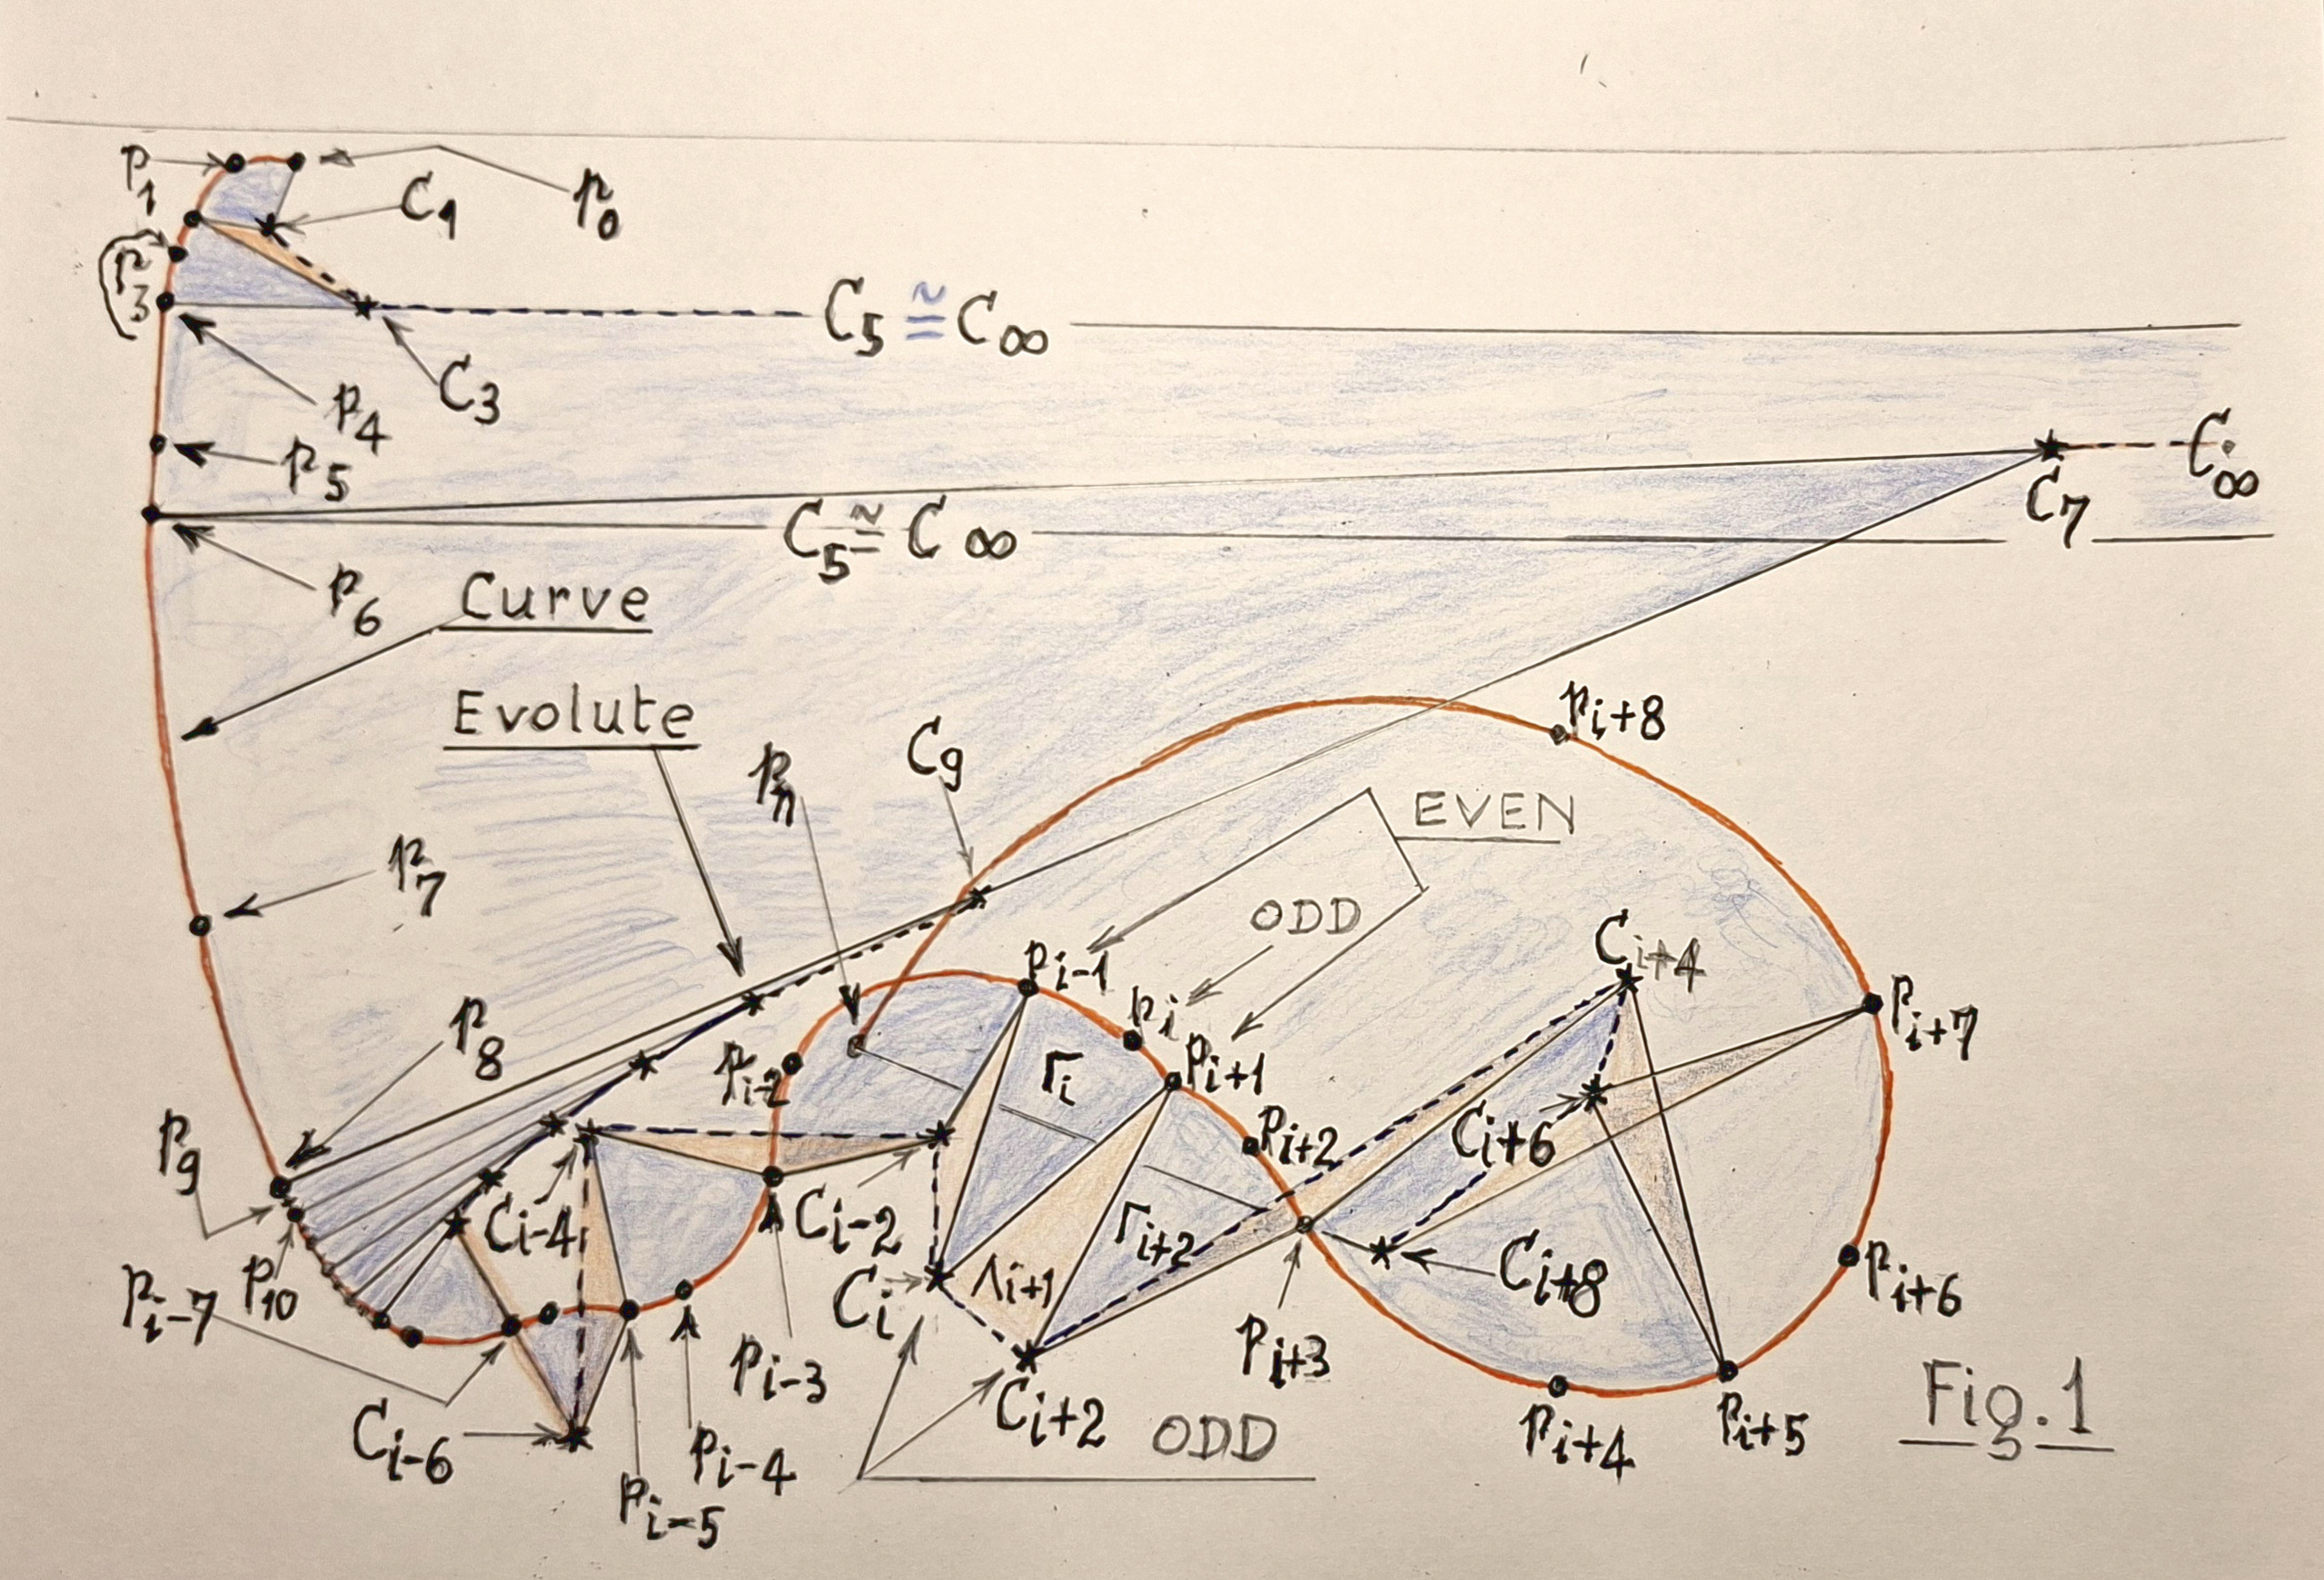
\includegraphics[angle=90,
                 width=\dimexpr\paperwidth-4cm\relax,
                 height=\dimexpr\paperheight-7cm\relax,
                 keepaspectratio]{drawings/trace-2.jpg}
\end{center}
\newpage


\noindent \textbf{Intrinsic Representation of a Trace by the \{Ensemble\}.}
 
\noindent An \{\,Ensemble\,\} = \{\,Curve \,, Evolute\,\} can represent a Trace.   

\noindent In the Representation, continuities and discontinuities of the Trace must be kept in the Ensemble. \qquad (5.1)

\noindent \textbf{Sequences.} In said Representation: a\,) for the Curve, a Sequence of Triads, three Marks for each Triad; b\,) for the Evolute, a Sequence  of Tripods, three Points for each Tripod, i.e. two Curvature Centers and one Even Mark.

\noindent Even Marks are Points of the Curve and of the \{\,Evolute Planes\,\}.\\ Curvature Centers are Points of the Evolute and of the \{\,Curve Planes\,\}.\\(\,That is, some sort of symmetry: Curve, Evolute\,). \qquad (5.2) 

\noindent Ordered Aggregates in the Ensemble: \{\,Terns\,\}, \{\,Triplets\,\}. \qquad \qquad (5.3)

\noindent \textbf{\{\,Tern\,\}.} In the Ensemble, a \{\,Tern\,\} is any oriented aggregate:\\ \big\{\;\{Previous Curve Triangle\}\;,\;\{Evolute Triangle\}\;,\;\{Next Curve Triangle\}\;\big\}.

\noindent Where Previous, Next are with reference to the \{Evolute Triangle\}.

\noindent Only one Mark, that is an EM, in common to the Tern's three Triangles. 

\noindent Generally a Tern is in $\mathbb{R}^{\,3}$\,. Say: 

\noindent \{Tern\}$_{\,i-1}$\,=\,\big\{\,\{Curve\,Triangle\}$_{\,i-2}$\,,\,\{Evolute\,Triangle\}$_{\,i-1}$\,,\,\{Curve\,Triangle\}$_{\,i}$\,\big\} = $\{\,\Gamma_{\,i-2}\;,\;\Lambda_{\,i-1}\;,\;\Gamma_{\,i}\,\}$\,. \; With:\; $\Gamma_{\,i-2}\;\supset\;C_{\,i-2}$\;. $\Lambda_{\,i-1}\,\supset\;\{\;C_{\,i-2}\;,\;C_{\,i}\;\}$\;. $\Gamma_{\,i}\;\supset\;C_{\,i}$\,. Generally:\; $C_{\,i-2}\;\neq\;C_{\,i}$\,. For the common Even Mark = $p_{\;i-1}$\,: $\Gamma_{\,i-2} \supset p_{\,\to\,(i-1)}$\;\,;\,\;$\Lambda_{\,i-1} \supset p_{\,i-1}$\;\,;\,\;$\Gamma_{\,i} \supset p_{\,(i-1)\,\to}$\,. \qquad(5.4)

\noindent A Rotation along $B$ in any single \{Curve Triangle\}.\\\{\,Terns\,\} are introduced to evaluate Rotations in the entire $\mathbb{R}^{\,3}$\,. \qquad (5.5) 

\noindent \textbf{Tern's properties.} In a Tern, the \{Previous Curve Triangle\} yields its intrinsic properties. The \{Next Curve Triangle\} yields its intrinsic properties. Their intermediate \{Evolute Triangle\} yields \textsl{the two \{Curve Triangles\}' relative properties.} \qquad \qquad (5.6)

\noindent \textbf{In each Tern, a sequence:}\\ \{Curve's Previous Arc\}, EM, \{Curve's Next Arc\}.\\ Note. One EM between two Arcs avoids the following inconveniences.\\ 1\,] The partial superposition of two non-pointlike Arc Intervals, and the ensuing necessary of getting, from these two Arc Intervals, a necessarily unique, chosen Curve's Interval.\\ 2\,] The impossible representation of Abrupt Rotations in the Curve. \qquad (5.7)

\noindent \textbf{\{\,Terns\,\}.}\,The ordered set \{\,Terns\,\} is used to analyze the entire Ensemble.  (5.8)

\noindent \textbf{Two main subsets:} \quad \{\,Abrupt Terns\,\}, \{\,Differential Terns\,\}. \qquad (5.9)

\noindent \textbf{\{\,Abrupt Tern\,\} i.e. Jump.}

\noindent The \{Evolute Triangle\}, say $\Lambda_{\,i-1}$\,, by definition having one Mark i.e. \{\,EM\,\} = $p_{\;i-1}$ only, not a Curve's Interval, expresses a Jump at said\\ $p_{\;(i-1)} = p_{\,\to\,(i-1)}\,\cup\,p_{\,(i-1)\,\to}$\, if\\ $T_{\;\to\;p_{\;(i-1)}} \neq T_{\;p_{\;(i-1)}\,\to} \vee N_{\;\to\;p_{\;(i-1)}} \neq N_{\;p_{\;(i-1)}\,\to} \vee B_{\;\to\,p_{\;(i-1)}} \neq B_{\;p_{\,(i-1)}\,\to}\,, \vee$ a composition of them. That implies: $C_{\,i-2} \neq C_{\,i}$\,. There is not a continuous \{\,Evolute's Arc\,\}\,. i. e. there are undefined Centers in the Interior of the Interval $[\;C_{\,i}\,-\,C_{\,i-2}\;]$\,. \qquad \qquad (5.10)

\noindent  \textbf{Tern Cases.} For the Tern $\big\{\;\Gamma_{\,i}\;,\;\Lambda_{\,i+1}\;,\;\Gamma_{\,i+2}\;\big\}$. \qquad (\,For these cases, the Frenet-Serret frames shall be analyzed in a following subsection.\,) 

\noindent Case 1.\quad\{\,Curve Triangles\,\}  \; $\Gamma_{\,i} \neq \Gamma_{\,i+2}$\,.

\noindent \{\,Evolute Triangle\,\} = $\Lambda_{\,i+1}\;\supset\;\big\{\;p_{\;i+1}\;,\;C_{i}\;,\;C_{i+2}\;,\;\;R_{\,(i+1)\;(i)}\;,\;R_{\,(i+1)\;(i+2)}\;\big\}$.

\noindent \{\,Curvature Centers\,\} = $\{\;C_{\,i}\;,\;C_{\,i+2}\;\}$\,; \{\,EM\,\} = $p_{\,i+1}$\;;\; For $\Lambda_{\,i+1}$\,:\\Initial Vector Ray =  $R_{\,(i+1)\,(i)}\;=\;[\,p_{\,i+1}\,-\,C_{\,i}\,]$\;\,;\\Final Vector Ray = $R_{\,(i+1)\,(i+2)}\;=\;[\,p_{\,i+1}\,-\,C_{\,i+2}\,]$\,.\qquad \qquad (5.11)

\noindent Case 2. A special case. \;\{\,Curve Triangles\,\} \; $\Gamma_{\,i} \neq \Gamma_{\,i+2}$\,. They are non-coplanar, and with curvatures having same values.\\ The \{Evolute Triangle\} = $\Lambda_{\,i+1}$ is an \textbf{Edge} between them. On this Edge: \\$R_{\,(i+1)\,(i)} = R_{\,(i+1)\,(i+2)}\;;\;||\,R_{\,(i+1)\,(i)}\,|| = ||\,R_{\,(i+1)\,(i+2)}\,||\;;$\;;\;$C_{\,i} = C_{\,i+2}$\,. (5.12) 

\noindent Case 3. A special case. \{\,Curve Triangles\,\} \;$\Gamma_{\,i} \neq \Gamma_{\,i+2}$\,. They are non-coplanar, and with different curvatures.\\ The \{Evolute Triangle\} = $\Lambda_{\,i+1}$\, is an \textbf{Edge} between them. On this Edge:\\ $R_{\,(i+1)\,(i)} \neq R_{\,(i+1)\,(i+2)}$\,;\;$||\,R_{\,(i+1)\,(i)}\,|| \neq ||\,R_{(i+1)\,(i+2)}\,||$\;;\;$C_{\,i} \neq C_{\,i+2}$\,.\qquad (5.13)

\noindent Case 4. A special case. \{\,Curve Triangles\,\} $\Gamma_{\,i} \neq \Gamma_{\,i+2}$\,. They are coplanar, but with different curvatures.\\The \{Evolute Triangle\} = $\Lambda_{\,i+1}$ is a \textbf{Segment} between them. On it:\\ $R_{\,(i+1)\,(i)} \neq R_{\,(i+1)\,(i+2)}$\;;\;$||\,R_{\,(i+1)\,(i)}\,|| \neq ||\,R_{\,(i+1)\,(i+2)}\,||\;;\;C_{\,i} \neq C_{\,i+2}$\,.\quad  (5.14) 

\noindent Case 5. A special case. Coplanar Triangles $\Gamma_{\,i}\;,\;\Lambda_{\,i+1}\;,\; \Gamma_{\,i+2}$\,. $\Gamma_{\,i} \neq \Gamma_{\,i+2}$\,. The \{\,Curve Triangles\,\} have equal scalar Radii,  different Vector Radii, different Curvature Centers. Between them, the \{Evolute Triangle\} = $\Lambda_{\,i+1}$ has: \,$R_{\,(i+1)\,(i)} \neq R_{\,(i+1)\,(i+2)}$\;;\;$||\,R_{\,(i+1)\,(i)}\,|| = ||\,R_{\,(i+1)\,(i+2)}\,||\;;\;C_{\,i} \neq C_{\,i+2}$\,.\quad (5.15)  

\noindent \textbf{Differential Triad.} 

\noindent In Math, a \textbf{\{\,Differential Interval between two Points\,\}} has a tiny value and can be assumed straight with reference to the local Scalar Radius.

\noindent This is not the case of a tiny Interval along a Trace; if not a \{\,Pair of Points\,\} is considered, but a \textbf{\{\,Differential Triad of Marks\,\}}, and this \{\,Triad of Marks\,\} implies
 a \{Differential Curve Plane\,\}, a \{\,Differential Curve Triangle\,\}, a \{\,Differential Curve Arc\,\} with generally non-null curvature. (5.16) 

\noindent \textbf{\{\,Differential Tern\,\}.} A \{\,Differential Tern\,\} has $0 \vee 1 \vee 2$ \{\,Differential Curve Triangles\,\} and, among them, one \{\,Differential Evolute Triangle\,\}.

\noindent For any \{\,Differential Tern\,\} it is admissible to assume in the Evolute a small, straight by no further knowledge\\ \{\,Evolute's Arc\,\} = $[\;C_{\;Next\;Curve\;Arc}\,-\,C_{\;Previous\;Curve\;Arc}\;]$\,. \qquad \qquad (5.17)

\noindent \textbf{Sequence \{\,Differential Terns\,\} corresponding to an Ensemble's Interval.}

\noindent The necessity that an Interval of the Ensemble be a Sequence of 1st Differential Subintervals is the strong and smooth variation of Curvature in the corresponding Trace. In this Ensemble's Interval, the Sequence \{\;Differential Terns\;\} is at the Human's discretion. A good Representation of this Interval implies a high density of Curve's Marks. Unfortunately, a high density of Marks corresponds to a big set of measured distances\, $dv$ (\,in the program\,). (5.18)

\noindent That is, the Human introduces in the Ensemble a numerous Sequence of tiny \{\,Curve Triangles\,\}, each one with a very short Arc, and of tiny \{\,Evolute Triangles\,\}, each one with two very near Centers of curvature.\qquad (5.19)

\noindent In any \{Differential Curve Triangle\} the \{\,Differential Triad\,\} has one tiny Arc with a specified Curvature Center. Hence this Arc, although tiny, is not a Straight Segment. But two Differential Arcs compose this tiny Arc; they can be assumed straight, since Scalar Radius > > Differential Arc's Length. \qquad (5.20)

\noindent What is the consequence of an eventual badly approximate representation of this Ensemble Interval? \textsl{It is a local imprecise correspondence of this Ensemble's Interval with that of a more precisely measured Ensemble's Interval.} \qquad (5.21) 

\noindent In a Sequence \{\,Differential Terns\,\}:
 
\noindent \textbf{a) Initial Differential Tern.} The supposedly given \{Initial Curve Triangle\} has a finite Arc-length. It is followed by a \{Differential Evolute Triangle\} with two very near Curvature Centers. It is followed by a \{Differential Curve Triangle\} with a tiny Arc-length. \qquad \qquad (5.22)

\noindent \textbf{b) A numerous set \{\,Differential Intermediate Terns\,\}} may occur.

\noindent A \{\,Differential Intermediate Tern\,\} is composed by:\\ \{Previous Curve Triangle\} with tiny Arc-length;\\\{Differential Evolute Triangle\} with two very near Curvature Centers;\\\{Next Curve Triangle\} with tiny Arc-length. (5.23) 

\noindent \textbf{c) Final Differential Tern.} The \{Previous Differential Curve Triangle\} has a tiny Arc-length. It is followed by a \{Differential Evolute Triangle\} with very near Curvature Centers. It is followed by the \{Final Curve Triangle\} with a finite Arc-length. \qquad \qquad (5.24)

\noindent An \{\,Ensemble's Interval\,\} corresponds to the above\; a - b - c. \qquad  (5.25) 

\noindent \textbf{Rotation.} A "Rotation" is short for "Rotation angle" .\\It is around a specified Axis that is across a specified Point.
\\In a \{Curve Triangle\}, of the Outgoing Vector Radius with reference to the Incoming Vector Radius.\\In a \{\,Tern\,\}, of the \{Next Curve Triangle\} with reference to the \{Previous Curve Triangle\}. \qquad \qquad (5.26) 

\noindent \textbf{Rotation classes.}

\noindent \textbf{Class by \{\,t\,\}.}

\noindent a\,] Abrupt Rotations.\quad Implying a (\,t\,) value. \qquad (5.27)

\noindent b\,] Differential Rotations. Implying a tiny Interval\; $\Delta\,t\;\vee\;\delta\,t$\, \qquad (5.28)

\noindent c\,] A definite Rotation, implying a finite Interval. (5.29)                      

\noindent \textbf{Class by Axis.}

\noindent d\,] Around a specified Axis across the ${\{\,Curvature\;Center\,\}}$ of the \{\,Curve Triangle\,\}.\qquad(5.30). 

\noindent e\,] Around a specified Axis across the EM of the reference \ {\,Previous Curve Triangle\,\} of a \{\,Tern\,\}. \qquad (5.31)
           
\noindent \textbf{\{T,\,N,\,B\} and \{\,D\,C\,M\,\}.} \,Any Rotation in the field \{\,T,\,N,\,B\,\} is expressed by the  \{\,Direction Cosine Matrix\,\} = \{\,D\,C\,M\,\}.\, \{\,D\,C\,M\,\} encodes \{\,T,\,N,\,B\,\} consistently.\qquad(5.32)

\noindent \textbf{Basic Rotations within a \{\,Curve Triangle\,\}.}

\noindent \textbf{Case c1.} In a \{Curve Triangle\}, say $\Gamma_{\,i}$\,, of which the Interior is considered. The constant Curvature that is associated to the scalar Radius and to the Vector Radii, is also associated to a Rotation angle, around the, constant in $\Gamma_{\,i}$\,, Unit Binormal Vector \{\,B\,\}$_{\,C_{\,i}}$ at the constant Curvature Center $C_{\,i}$:\, of the \{Incoming to the Arc's Final Mark Vector Radius\} relative to the \{Outgoing from the Arc's Initial Mark Vector Radius\}\,. It is the geometric Angle at $C_{\,i}$ of the \{Curve Triangle\} = $\Gamma_{\,i}$. Obviously, it is not an Abrupt Rotation.

\noindent \{\,Rotation Angle\,\} = $\nu\;B_{\,C_{\,i}}$\,, in the\\ \big(\,Int Arc\,\big)$_{\,i} = \big(\;p_{\;i-1}\to\;,\;...\;,\;p_{\,i}\;,\;...\;,\;\to p_{\;i+1}\;\big)$\,,

\noindent of the, incoming to the Arc's Final Mark, $T_{\,\to\,p_{\,i+1}}$\\ relative to the, outgoing from the Arc's Initial Mark, $T_{\,p_{\;i-1}\,\to}$ \;;

\noindent of the, incoming to the Arc's Final Mark, $N_{\,\to\,p_{\,i+1}}$\\ relative to the, outgoing from the Arc's Initial Mark, $N_{\,p_{\;i-1}\,\to}$\,. \qquad \qquad (5.33) 

\noindent \textbf{Abrupt Rotations at an EM.}

\noindent A definition: \textsl{Abrupt Rotations at an EM occur sharply, at the Parameter Value (\,t\,) of the EM.} \; Abrupt Rotations are not Differential Rotations.

\noindent An Abrupt Rotation at an EM may imply, but not necessarily: 1\,] Change of Curvature Center. 2\,] Change: previous Arc's Scalar Radius, next Arc's Scalar Radius. 3\,] Change: \{Incoming Vector Radius\}, \{Outgoing  Vector Radius\}. 4\,] Change: Incoming Frenet-Serret frame, Outgoing Frenet-Serret frame.\\ Possible Abrupt Rotations: 4.1\,] around \{T\}$_{\to EM}$\,; 4.2\,] around \{N\}$_{\to EM}$ i.e. a Torsion; 4.3\,] around \{B\}$_{\to EM}$ (\,please note: not around \{B\}$_{\,C}$\,)\,; 4.4\,] a composition of these Elemental Rotations.\qquad (5.34) 

\noindent The Curve has Parameter \{t\}; the Evolute has not an additional Parameter. In an Abrupt Rotation at an EM, which has a specified (\,t\,), the Evolute's Interval is \textsl{specified} only by its two end Points. \qquad \qquad (5.35)

\noindent \textbf{\{\,T, N, B\,\}$_{\,EM}$.} \; In a Tern, say $\big\{\;\Gamma_{\,i}\,,\;\Lambda_{\,i+1}\,,\;\Gamma_{\,i+2}\;\big\}$ with its central \\EM = $p_{\;(i+1)}$ = $\to\,p_{\;(i+1)}\;\,\cup\;\,p_{\;(i+1)}\,\to$\;, \;an Abrupt Rotation implies:\\incoming into EM, from the \{Previous Curve Triangle\}\;$\{\,T,\,N,\,B\,\}_{\,\to\,p_{\,(i+1)}}\;\neq$\\outgoing from EM to the \{Next Curve Triangle\}\; $\{\,T\,,\,N\,,\,B\,\}_{\,p_{\,(i+1)}\,\to}$\,. (5.36) 

\noindent \textbf{\{\,T, N, B\,\}$_{\,EM}$ and \{\,D\,C\,M\,\}$_{\,EM}$.} At said EM = $p_{\;(i+1)}$\,, the orientation of the outgoing \{T, N, B\}$_{\,p_{\;(i+1)}\,\to}$ relative to the incoming \{T, N, B\}$_{\,\to\;p_{\;(i+1)}}$ is defined by 9 Angles, equivalently by the \{\,Direction Cosine Matrix\,\}$_{\,p_{\;(i+1)}}$ = \{\,D\,C\,M\,\}$_{\,p_{\;(i+1)}}$\,. (\,\textsl{Not only by Curvature and Torsion}\,). \qquad \qquad \qquad (5.37)

\noindent \textbf{Basic Rotations around an Axis at an EM, hence Abrupt Rotations.} Say at the EM = $p_{\;i+1}$\, of the Tern $\{\,\Gamma_{\,i}\;,\;\Lambda_{\;i+1}\;,\;\Gamma_{\,i+2}\,\}$\,. Basic means around\, $T\,\vee\,N\,\vee\,B$\,. \qquad (5.38)

\noindent \textbf{Case d1.} \{\,Tern\,\} = $\big\{\;\Gamma_{\,i}\,,\,\Lambda_{\,i+1}\,,\,\Gamma_{\,i+2}\;\big\}$\,. A special case.

\noindent \{Evolute Triangle\} = $\Lambda_{\,i+1} \perp \Gamma_{\,i}\;,\;\Lambda_{\,i+1} \perp \Gamma_{\,i+2}$\,. That is $\Lambda_{\;i+1}\,\perp\,T_{\;\to\,p_{\;(i+1)}}$\,.

\noindent $\Lambda_{\,i+1}$'s boundary\;$\supset\;R_{\,(i+1)\,(\,i\,)}\,,\;R_{\,(i+1)\,(i+2)}$ with $||\,R_{\,(i+1)\,(i)}\,||\,=\,||\,R_{\,(i+1)\,(i+2)}\,||$\,; their tips at \;$p_{\,i+1}$\;;\;$C_{\,i}$ root of $R_{\,(i+1)\,(i)}$\,,\;$C_{\,i+2}$ root of $R_{\,(i+1)\,(i+2)}$\,. $C_{\,i} \neq  C_{\,i+2}$\,.  

\noindent $T_{\,p_{\,(i+1)}}\;=\;T_{\,\to\,p_{\,(i+1)}}\;\cup\;T_{\,p_{\,(i+1)}\,\to}$ = incoming $T_{\;p_{\,(i+1)}}\;\cup$ outgoing $T_{\;p_{\;(i+1)}}$\,. $T_{\;p_{\,(i+1)}}\;\perp\;\Lambda_{\,i+1}$\,. 

\noindent At $p_{\,(i+1)}$\, around \,$T_{\;\to\,p_{\,(i+1)}}$\,: \;
\{\,Rotation Angle\,\} = $\theta\;T_{\;p_{\,(i+1)}}$\,. \qquad 

\noindent $\theta$\, is the geometric Angle in $\Lambda_{\,i+1}$
\,at \,EM = $p_{\,(i+1)}$\\ of $\Gamma_{\,i+2}$ relative to\, $\Gamma_{\,i}$\,; visibly in the Curve of $A_{\,i+2}$ relative to $A_{\,i}$\,.
 
\noindent $\theta$ of $N_{\;p_{\,(i+1)}\,\to}$ relative to $N_{\;\to\,p_{\,(i+1)}}$\;\,;\,\;$\theta$ of $B_{\;p_{\,(i+1)}\,\to}$ relative to $B_{\;\to\,p_{\,(i+1)}}$\,. (5.39) 

\noindent \textbf{Case d2.} Let $\Lambda_{\,i+1}$ be an Edge between the non-coplanar $\Gamma_{\,i}$ and $\Gamma_{\,i+2}$; this Edge contains\; $R_{\,(i+1)\,(i)}\;\neq\;R_{\,(i+1)\,(i+2)}$\;;\; $p_{\;i+1}\;;\;C_{\,i}\;;\;C_{\,i+2}\;;\;C_{\,i} \neq C_{\,i+2}$\,. 

\noindent A Rotation around the Unit Vector $T_{\,C_{\,i}}$ is not for this case: its result should be a cut of the Curve at\, $p_{\;i+1}$\, and thr destruction of the Edge. \qquad (5.40)

\noindent \textbf{Case d3.} \{\,Tern\,\} = $\big\{\,\Gamma_{\,i}\,,\,\Lambda_{\,i+1}\,,\,\Gamma_{\,i+2}\,\big\}$\,. A special case.

\noindent The \{Evolute Triangle\} = $\Lambda_{\;i+1}$ is an \{Edge\} between the non-coplanar \{\,Curve Triangles\,\}:\, $\Gamma_{\,i}\;,\;\Gamma_{\,i+2}$\,.

\noindent $\Lambda_{\,i+1}$\, contains: $R_{\,(i+1)\,(i)}\;\neq\;R_{\,(i+1)\,(i+2)}\;;\;p_{\;i+1}\;;\;C_{\,i}\,,\,C_{\,i+2}\;;\;C_{\,i}\;\neq\;C_{\,i+2}$\,.

\noindent Null angle at $p_{\,i+1}$ of the degenerate \{\,Evolute Triangle\,\}.

\noindent On this Edge, parallel Unit Vectors: \; $N_{\;\to\,p_{\,(i+1)}}\;,\;N_{\;p_{\,(i+1)}\,\to}$\,.

\noindent The reference $N_{\;\to\,p_{\;i+1}}$ is across $p_{\;i+1}$ and also across $C_{\,i}$\,.

\noindent\{\,Rotation Angle\,\} = $\tau\;N_{\;\to\,p_{\;i+1}}$ = Abrupt Torsion\,;

\noindent $\tau$ of $\Gamma_{\,i+2}$ with reference to $\Gamma_{\,i}$\,.

\noindent At $p_{\;i+1}$\,: \,$\tau$\quad of \quad $T_{\;p_{\;i+1}\,\to}$\, re \,$T_{\;\to\,p_{\;i+1}}$\;;\quad of \quad $B_{\;p_{\;i+1}\,\to}$\, re \,$B_{\;\,\to\,p_{\;i+1}}$\,.\quad (5.41)

\noindent \textbf{Case d4.} Let $\Lambda_{\,i+1}$ be special: an Edge between the non-coplanar $\Gamma_{\,i}$ and $\Gamma_{\,i+2}$\,; this Edge contains\; $R_{\,(i+1)\,(i)}\;\neq\;R_{\,(i+1)\,(i+2)}\;;\;p_{\;i+1}\;;\;C_{\,i}\;;\;C_{\,i+2}$\;;\;$C_{\,i} \neq C_{\,i+2}$\,;  parallel Unit Vectors \; $N_{\;\to\,p_{\,(i+1)}}\;,\;N_{\;p_{\,(i+1)}\,\to}$\,.

\noindent \{\,Rotation Angle\,\} = Abrupt Torsion = $\tau \;N_{\,C_{\,i}}$\,. 

\noindent This case is equivalent to case d3; it has a different Point of application of Unit Vector $N$\,, that is\, $C_{\,i}$\,. \qquad (5.42)

\noindent \textbf{Case d5.} \{\,Tern\,\} = $\big\{\;\Gamma_{\,i}\,,\;\Lambda_{\,i+1}\,,\;\Gamma_{\,i+2}\;\big\}$\,. A special case.

\noindent The Tern's three Triangles are in the same Plane $\perp\,B_{\;p_{\;i+1}}$\,.

\noindent The \{Evolute Triangle\} = $\Lambda_{\,i+1}$\; contains:\\ EM = $p_{\;i+1}$\;;\\Curvature Centers \;  $C_{\,i}\;,\;C_{\,i+2}$\,;\\ Vector Radii \; $R_{\,(i+1)\,(i)}\;,\;R_{\,(i+1)\,(i+2)}$\,; in general \,$||\,R_{\,(i+1)\,(i)}\,|| \neq ||\,R_{\,(i+1)\,(i+2)}\,||$\,.

\noindent At \, $p_{\;i+1}$\,: \; \{\,Rotation Angle\,\} = $\psi\;B_{\,p_{\;i+1}}$\,.

\noindent $\psi$ \,is the geometric Angle of\, $\Lambda_{\,i+1}$ \,at its vertex \,EM = $p_{\;i+1}$\,.

\noindent $\psi$\, around $B_{\,p_{\;i+1}}$\, at \, EM = $p_{\;i+1}$ \,and not around $B_{\;C_{\,i}}$ at\, $C_{\,i}$ \,of $\Gamma_{\,i}$\,.

\noindent $\psi$\quad of \quad $T_{\,p_{\;i+1}\,\to}$\quad re \quad $T_{\,\to\,p_{\;i+1}}$\; ;\; $\psi$\quad of \quad $N_{\,p_{\;i+1}\,\to}$ \quad re \quad $N_{\,\to\,p_{\;i+1}}$\,.\;(5.43)

\noindent \textbf{Case d6.} \{\,Tern\,\} = $\big\{\;\Gamma_{\,i}\,,\;\Lambda_{\,i+1}\,,\;\Gamma_{\,i+2}\;\big\}$\,.It is a special case: the two \{\,Curve Triangles\,\} and the \{Evolute Triangle\} are coplanar and $\perp\,B_{\;C_{\,i}}$. $\Lambda_{\,i+1}$ contains:\; EM = $p_{\;i+1}$\;;\; $C_{\,i}\;,\;C_{\,i+2}$\;;\;$R_{\;(i+1)\,(i)}\;;\;R_{\;(i+1)\,(i+2)}$\,. 

\noindent A Rotation around the Unit Vector $B_{\;C_{\,i}}$ is not considered because its result is a cut of the Curve at $p_{\,i+1}$ and its destruction. \qquad (5.44)

\noindent \textbf{Differential Rotations}\,in a Sequence\,\{\,Differential Terns\,\}.\\A simple, sufficiently smooth example.

\noindent Let us consider the Sequence:\\ $\{\;\ldots\;,\;\Gamma_{\,i-2}\;,\;\Lambda_{\,i-1}\;,\;\Gamma_{\,i}\;,\;\Lambda_{\,i+1}\;,\;\Gamma_{\,i+2}\;,\;\Lambda_{\,i+3}\;,\;\Gamma_{\,i+4}\;,\;\Lambda_{\,i+5}\;,\;\Gamma_{\,i+6}\;,\;\ldots\;\}$\,. 

\noindent Where, in general, the \{\,Curve Triangles\,\} are non-coplanar and pairwise hinged along Segments.
 
\noindent \textbf{Finite} $A_{\,i-2} \subset \Gamma_{\,i-2}$\;.

\noindent \textbf{Tiny}\; $A_{\,i} \subset \Gamma_{\,i}$\;,\;$A_{\,i+2} \subset \Gamma_{\,i+2}$\;,\;$A_{\,i+4} \subset \Gamma_{\,i+4}$\,.

\noindent \textbf{Finite} $A_{\,i+6} \subset \Gamma_{\,i+6}$\;. 

\noindent To understand the case, in the above Sequence let us consider the Tern $\{\;\Gamma_{\,i}\;,\;\Lambda_{\,i+1}\;,\;\Gamma_{\,i+2}\;\}$. 
  
\noindent The \{Evolute Triangle\} = $\Lambda_{\,i+1}$ is the Segment containing: Vector Ray $R_{\,(i+1)\,(i)}$ , Vector Ray $R_{\,(i+1)\,(i+2)}\;,\;p_{\,i+1}\;,\;C_{\,i}\;,\; C_{\,i+2}\,,\,N_{\,(i+1)\,(i)}\,,\,N_{\,(i+1)\,(i+2)}$\,. \qquad (5.45) 

\noindent \textbf{\{Triplet\}}=\big\{\{Evolute Triangle\},\,\{Curve Triangle\}\,,\,\{Evolute Triangle\}\big\}.(5.46)

\noindent \textbf{\{\,Triplets\,\}.} For an Open Curve, \{\,Triplets\,\} are in the Interior only.\\For a Closed Curve, \{\,Triplets\,\} correspond to the entire Curve. (5.47) 

\section{Preliminary collection of data, by the Human.}

\noindent \textsl{Supposedly without an already given Parametrization in $\mathbb{R}^{\,3}$:}\\ the Marks' Cartesian Coordinates are not an input, but a Curve's property that the Human's and Program's operations pull out. \qquad \qquad  (6.1)

\noindent A preliminary work must be done:\; the Human must intrinsically define the\\ Ensemble: Curve \& Envelope, from the Trace. \qquad (6.2) 

\noindent It is said "intrinsically". Intrinsic to a part of $\mathbb{R}^{\,3}$\,. At first, this part is the \{\,Initial Reference Space\,\}. This part growns up to the \{\,Triangulation Nest\,\}, that envelops the Ensemble at the end of operations. \qquad \qquad \qquad (6.3)

\noindent \textbf{\{\,Initial Reference Space\,\}.} From the Marked Trace, a Curve ensues. For this Curve, an \{\,Initial Reference Space\,\} is conceived by the Human.

\noindent \textsl{She chooses four, not all coplanar Marks} on the Marked Trace. These Marks $\subset$ \{\,Marks\,\} assume the surnames\, \{\,Reference Marks\,\} = \{\,q0, q1, q2, q3\,\}.\quad (6.4)

\noindent That is, since the four \{\,Reference Marks\,\} (\,say $p_{\,m}\,,\,p_{\,r}\,,\,p_{\,g}\,,\,p_{\,h}$\,) are important, each one of them has a surname:\quad $p_{\,m}\,q0\;,\;p_{\,r}\,q1\;,\;p_{\,g}\,q2\;,\;p_{\,h}\,q3$\;.\qquad \qquad (6.5)  

\noindent Not necessarily the \{\,Reference Marks\,\} are a continuous interval of the \{\,Marks\,\} sequence. \qquad \qquad \qquad \qquad \qquad (6.6)

\noindent In the \{\,Initial Reference Space\,\}, the \{\,Reference Marks\,\} are the specified, assumed end terminals of the Human's measurements in $\mathbb{R}^{\,3}$ of four straight Distances, for any Mark (\,p\,) of \{\,Marks\,\}.  (6.7)

\noindent The \{\,Reference Marks\,\} are the vertexes of the, generally non-regular, \textbf{Reference Tetrahedron}. Obviously, not a degenerate Tetrahedron. ( For a plane Trace, an out-of-plane Segment is adjoined to an end of the Trace, giving hospitality to one out-of-plane Reference Mark. )\qquad(6.8)

\noindent The Human has a metering stick; she intrinsically measures 

\noindent \textbf{\big\{\,Distances:\, \{Marks\}<-->\{Reference Marks\}\,\big\}:}

\noindent Matrix $\,dv$ = $\big\{\;\forall\;p\;;\;\; ||\,p - q0\,||, ||\,p - q1\,||, ||\,p - q2\,||, ||\,p - q3\
,||\;\big\}$. \qquad (6.9)

\noindent Completing the Matrix\, \{\,Indexed Marks; Marks' Distances\,\} = $dv$ \,the Human gets an Intrinsic Definition of the Array \{\,Marks\,\}, relative to the Curve's \{\,Initial Reference Space\,\}. \qquad (6.10) 

\noindent For any specified Mark (\,p\,) of the Array \{\,Marks\,\}, in general 4 non-null \{\,Mark's Distances\,\}$_{\,p}$ correspond. 3 non-null and a null one if the examined Mark (\,p\,) coincides with one of \{\,q0, q1, q2, q3\,\}.\qquad \qquad (6.11)

\noindent Within the set \{\,Distances\,\}, there are the six\\ \{\,Reference Distances among the Reference Marks\,\} =

\noindent $\big\{\,d01 = ||\,q0 - q1\,||,\; d12 = ||\,q1 - q2\,||,\; d20 = ||\,q2 - q0\,||,\; d03 = ||\,q0 - q3\,||,\; d13 = ||\,q1 - q3\,||,\; d23 = ||\,q2 - q3\,||\,\big\}$\,.\qquad \qquad (6.12)

\noindent \textbf{Hints.}

\noindent The subset \{\,Reference Marks\,\} is preferably  chosen near the Curve's approximate center of gravity, aiming to the containment of the lengths of the set\\ =\{\,Marks' Distances\,\} = \big\{\,Distances: \{Marks\} <--> \{Reference Marks\}\,\big\} $\subset dv$. \qquad (\,Hint 1\,) \qquad (6.13)

\noindent It is advisable to choose far apart \{\,q0, q1, q2, q3\,\}: their spread increases precision of the measurement. \qquad \qquad \qquad \qquad (\,Hint 2\,) \qquad (6.14)

\noindent A substantial non\,-\,planarity of \{\,q0, q1, q2, q3\,\} helps to get rid of the Marks' Mirror Images. \qquad \qquad \qquad \qquad (\,Hint 3\,) \quad (6.15)

\noindent If the Curve's No. of Marks is ${N}_{\,M}$\,, then\, $Number_{\,Distances} \approx 4\,N_{\,M}$\,.\; (6.16)   

\noindent Each Mark's measurement is independent from the other Marks'measurements, not independent from the measurements of the considered Reference Mark, obviously.\textsl{There is not a succession of dependent measurements along the marked Trace.} \qquad (6.17)  

\noindent The Human stores the Matrix\, \{\,Indexed Marks\,; Marks' Distances\,\} = $dv$ \,in order to give it to CPlanes.py. \qquad (6.18)

\noindent \textbf{Marked Trace's handedness}: a left - handed Trace must be represented by a left - handed Curve, and a right - handed Trace by a right - handed Curve. \qquad (6.19)

\noindent Left and Right are ascertained on a chosen \{\,Handedness Reference Interval\,\} of the marked Trace, since, in general, the marked Trace may have left and right-handed parts in sequence, and so the ensuing Curve.  \qquad \qquad (6.20)

\noindent The Human acknowledges the marked Trace's handedness and defines the corresponding parameter "Handedness". \quad (6.21)

\noindent \{\,Reference Marks\,\}, \{Reference Distances\,\} and "Handedness" are defining properties of the ensuing Ensemble. \qquad \qquad (6.22)

\section{The Human and CPlanes. py}  

\noindent The Human communicates: \{Reference Marks\}, \{Reference Distances\}, \{Indexed Marks\,; Marks' Distances\}, "\,Handedness\," to the program CPlanes.py. 

\noindent \textbf{The 1st intervention of CPlanes. py.} If the program CPlanes py is at the Human's disposal, it helps; CPlanes. py can determine:

\noindent The Cartesian axes:\; x, y, z\,  across q0. \qquad \qquad \qquad (7.1)

\noindent The Reference Marks' coordinates:\\q0(\,0, 0, 0)\,;\, q1(\,d01, 0, 0\,)\,;\, q2(\,x(q2), y(q2), 0)\,;\, q3(\,x(q3), y(q3), z(q3)\,).

\noindent q1 lies on the positive x axis.

\noindent q2 lies in the x\,y plane with y(q2)\,>\,0.

\noindent Handedness = "right" gives z(q3)\,>\,0.

\noindent Handedness = "left" gives z(q3)\,<\,0. \qquad (7.2)

\noindent By them, the Human gets a coordinated \{\,Initial Reference Space\,\} $\subset\;\mathbb{R}^{\,3}$\,.  

\noindent It is the \{\,Inital Reference Space\,\} because it shall be implemented again, getting the \{\,Triangulation Nest Reference Space\,\} that envelops the Ensemble. (7.3)

\noindent \textbf{The 2nd intervention of CPlanes. py.} CPlanes.py effects the Reconstruction of any Mark p $\in\;dv$ by 4 Trilaterations by the 4 Triples \big\{\,\{q0, q1, q2\}, \{q0, q1, q3\}, \{q0, q2, q3\}, \{q2, q1, q3\}\,\big\} of the Tetrahedron.\qquad (7.4)

\noindent For each \,p\,, each Trilateration - one Triple - \{\,three Distances\,\} - yields two \textsl{Solutions}:\; one, and its Mirror Image. \qquad (7.5)

\noindent For each p\,, the 4 Trilaterations yield\; 8 \textsl{Solutions} . \qquad (7.6)

\noindent For each \,p\,, the array \{\,Candidates\,\}$_{\,p}$ stores the Solutions. \qquad (7.7)

\noindent  By the array\{\,accepted\,\}:

\noindent For each \,p\,, CPlanes.py does the Validation, i.e. the \textsl{selection}:\\ accepted $\vee$ inconsistent $\vee$ ambiguous\; \textsl{Position p.}\; \;  (7.8)

\noindent For each\, p\,, CPlanes.py chooses the best Candidate Position, naming it the "\,reconstructed p\,", \textsl{gives its Coordinates}, and discards the Mirror Images. (7.9)

\noindent For each\, p\,, it is sufficient one false Distance$_{\,p}$ of 4 to contaminate 3 Distances$_{\,p}$ and render suspect all 4 Distances$_{\,p}$. Result: a Human's new measurement of 4 Distances$_{\,p}$ is needed. \qquad \qquad (7.10)

\noindent The above, $\forall\;p\;\in\;dv$\,. \qquad \qquad (7.11)

\noindent Hence CPlanes.py gives the  Matrix \{\,Coordinates\,\} for $dv$. (7.12)

\noindent The above is distance-geometry with redundancy. It is over-determined by purpose.\qquad \qquad (7.13) 

\noindent \textbf{Notice.} Said interventions of CPlanes.py have an argument: the set \{\,Indexed Marks\,\} of the Curve, not all \{\,Points\,\} of the Curve. The Curve's Arcs, and their - Arc-defined - \{\,Extra Points\,\} are not yet specified, hence not yet considered at this stage. By the above data it is not yet possible to draw sufficiently satisfying plots of the Curve. \qquad \qquad (7.14)

\noindent \textbf{The 3rd intervention of CPlanes.py.}

\noindent \{\,Arcs\,\}, \{\,Extra Points\,\} are calculated. \qquad \qquad (7.15)

\noindent \textbf{The 4th intervention of CPlanes.py: Plots.}

\noindent CPlanes.py can produce for a Curve:

\noindent a\,] The Curve's Plot, with Indexed Marks, Curvature Centers, Boundary Vector Radii, Arc-based densification by Extra Points.

\noindent b\,] At any Mark, for the Outgoing Frenet Serret frame, with reference to the Incoming Frenet Serret frame, 3 Plots:\\ T comparison, N comparison, B comparison. \qquad \qquad (7.16)    

\noindent \textbf{Planar Trace.} A planar Trace is managed by adjoining  one out-of-plane Segment to one of its ends. 

\noindent \textbf{Appendices}

\noindent \textbf{Appendix A}
The full Python source code for CPlanes class is here:

  https://github.com/giuse/trace/CPlanes.py

\noindent \textbf{Appendix B}
The Plot of bare Curve 8 and its 3 Plots: T comparison, N comparison, B comparison. 
 
\noindent The Plots of: Curve 4, Curve 11 are available. 

\qquad \qquad \qquad \qquad \qquad \qquad \textbf{Acknowledgements}

\noindent Many thanks for his invaluable help to\, Marco Solari, I.T.C., my Information Advisor; to\, ChatGPT and its team, for the program, suggestions and continuous assistance.  

\end{document}